% https://journals.aps.org/prl/abstract/10.1103/PhysRevLett.106.073005 lattice clock ref

% https://journals.aps.org/prl/abstract/10.1103/PhysRevLett.127.100401

% %  If using typographer caps, consider starting with an O or an S as these are visually quit striking - the H and R are also quite good


% % Preamble: A short list of key references/reviews for the student


\chapter{Theoretical background}
\markboth{\thechapter. THEORETICAL BACKGROUND}{}
\label{chap:theory}
	\begin{adjustwidth}{0cm}{0cm}
	\begin{flushright}
	\singlespacing
	\emph{``No one's mouth is big enough to utter the whole thing."\\} 
	- Alan Watts
	\end{flushright}
	\end{adjustwidth}
	\onehalfspacing
	\vspace{1cm}


	\noindent{A} cold atom experimentalist draws on a panoply of tools (both conceptual and instrumental) which are all intricate and absorbing in their own right.
	This chapter presents the essential ideas needed to give form and context to the content of the major works reported in this thesis.
	We will glance at the hydrogen atom to establish a language in which to elucidate the deceptively simple structure of helium.
	 We must be equipped with some study of the coupling between electromagnetic fields and light, given the ubiquitous use of laser sources and magnetic trapping in this dissertation, and the focus on laser spectroscopy\footnote{The \emph{focus} of a lens or mirror is the point of maximum concentration of light that is refracted or reflected from a distant or uniform source.
	Originally, the term referred to the fireplace at the centre of traditional single-room dwellings; still the brightest point of light, but also the source itself.}.
	Of course, the fun doesn't end when the lights turn off: Even in the dark, helium exhibits explosive two-body interactions, which impose limits on the size and lifetime of atomic condensates.
	Finally, we will review the basic features of the emergence of macroscopic coherence in the form of a Bose-Einstein condensate.
	
	% \footnote{A neophyte physicist may feel a compulsion to delve even deeper, under the weight of one's curiosity.
	% It bears reflecting on the caveat that knowledge is not power but potential energy: One has to do real work to realize that potential.}.
	
	% on colons: I thought that complete sentences get capitalized, elaborations don't

\section{Atoms and light}
\label{sec:atoms_and_light}
	The discussion in this section is a short tour of the relevant atomic physics.
	Many high-quality textbooks go into much greater detail than is required for this thesis and the reader is referred to, for example \cite{FootAtomic,BinneyBook} for deeper coverage.
	In this section, only the essential points are presented, omitting lengthy calculations, with references provided for the complete working.
	Our picture of atoms, their structure, and the interaction with electromagnetic fields, will be made in terms of their modern description in the language of quantum mechanics.

	Quantum mechanics is the study of systems whose state at any time $t$ is completely specified by a wavefunction $\ket{\psi(t)}$ and whose dynamics are determined by the time-dependent Schr\"{o}dinger equation,
	\begin{equation}
		i\hbar\frac{\partial}{\partial t}\ket{\psi(t)} = \hat{H}\ket{\psi(t)}.
		\label{eqn:TDSE}
	\end{equation}
	The wavefunction $\ket{\psi}$ is represented by a \emph{state vector} that is an element of the complex Hilbert space $\mathcal{H}$.
	The \emph{Born rule} postulates that the probability of a quantum system being observed in the state $\ket{\psi}$ given that it is known to be in the state $\ket{\phi}$ is given by squared inner product $|\braket{\psi}{\phi}|^2$.
	States are orthogonal if the inner product is zero, but the system may evolve naturally from $\ket{\phi}$ to have a nonzero projection onto $\ket{\psi}$ under the action of $\hat{H}$.
	The Hamiltonian $\hat{H}$ is a linear operator with the Hermitian property $\hat{H}^\dagger=H$, where the dagger denotes the conjugate transpose operation\footnote{Formally, $\mathcal{H}$ is a vector space $\mathbb{C}^D$ of dimension $D$ which is complete with respect to the $L^2$ norm $||x||=\sqrt{\braket{x}{x}}$ induced by the inner product $\braket{x}{y}\rightarrow\mathbb{C}$, and $\hat{H}\in\mathcal{B}$, the Banach space of bounded linear operators $\hat{O}:\mathcal{H}\rightarrow\mathcal{H}$.
	$\mathcal{B}$ is also a vector space with a norm (the trace norm) but not an inner product.
	The states themselves are defined up to scalar multiplication, and hence are actually rays in $\mathcal{H}$ better thought of as points in projective space; we will simply assume they are normalized as $\bra{\psi}\psi\rangle=1$ for brevity.
	We will say no more of the consternations stemming from the Born rule.}.	
	The Hermitian property guarantees $\hat{H}$ is \emph{normal}, $[\hat{H}^\dagger, \hat{H}]=0$ and therefore the time-independent Schr\"{o}dinger equation
	%mark
	\begin{equation}
		\hat{H}\ket{\psi} = E\ket{\psi}
		\label{eqn:TISE}
	\end{equation}
	specifies the eigenvectors $\ket{e_n}$ of $\hat{H}$ which provide a complete orthonormal basis for $\mathcal{H}$.
	This allows any (pure) quantum state to be written in the form $\ket{\psi} = \sum_n a_n\ket{e_n}$, with complex coefficients $a_n$ called \emph{amplitudes}.
	An interpretation of this fact in the light of the Born rule is that the energy eigenstates $\ket{e_i}$ correspond to distinguishable  and mutually exclusive  states of a system, which can be discriminated if their energy eigenvalues $E_i$ are different.
	% In the cases where eigenvalues coincide, there exists at least one other observable that could distinguish the degenerate energy eigenstates.
	
	
	The energy eigenbasis for a single charged particle bound in a central potential\footnote{Better known as the hydrogen atom.} have the form,
	\begin{equation}
	\psi_{nlm}(r,\theta,\phi) = 
	\sqrt{\left(\frac{2}{na_0 ^*}\right)^3\frac{(n-l-1)!}{2n(n+l)!}}e^{-\rho/2}\rho^l L_{n-l-1}^{2l+1}(\rho) Y^{m}_{l}(\theta,\phi)
	\end{equation}
	when written in spherical coordinates $(r,\theta,\phi)$, where $\rho = 2r/na_0 ^*$ and $a_0 ^* = \frac{4\pi\epsilon_0 \hbar^2}{\mu e^2}$ is the reduced Bohr radius.
	The radial Laguerre polynomials $L_{n-l-1}^{2l+1}(\rho)$ and the spherical harmonics $Y_{l}^{m}(\theta,\phi)$ are labeled by the angular momentum $l$, the magnetic quantum number $m$, and the energy is fixed by the principal quantum number $n$ as $E_n = -hcR_\infty/n^2$, where $h$ is the Planck constant, $c$ is the speed of light, and $R_\infty$ is the Rydberg constant.
	The bound-state energy $E_n$ is negative - one must do work to ionize the atom and produce the free ion-electron pair whose energy is defined to be zero.
	The quantum numbers $l$ and $m$ distinguish states that are otherwise degnerate in $n$, and the latter serve to lift the degeneracy via the Zeeman shift as I discuss in a later section.
	Here,  $h=2\pi\hbar$ is the Planck constant, $\varepsilon_0$ is the electric permittivity of free space, and $\mu$ is the Bohr magneton.
	
	

	Let us consider an atom immersed in an electric field oscillating with frequency $\omega = 2 \pi f$ (with $f$ in Hz), and write the Hamiltonian in the form
	\begin{equation}
		\hat{H}(t) = \hat{H}_0 + \hat{H}_{I}(t)
	\end{equation}
	where the bare atomic Hamiltonian $H_0$ sets the energy scale of the system, and the monochromatic time-dependent perturbation takes the form $\hat{H}_I(t) = \Lambda \cos(\omega t)$.
	We will give physical meaning to $\Lambda$ in a moment.
	The time-dependent state can be written in terms of the eigenbasis $\ket{\psi_n}$ of $\hat{H}_0$,
	\begin{equation}
		\ket{\Psi(t)} = \sum_n c_n(t)e^{-i\omega_n t}\ket{\psi_n},
	\end{equation}
	where $\omega_n= E_n/\hbar$.
	Substitution into Eqn \ref{eqn:TDSE} reduces to the coupled set of differential equations 
	\begin{equation}
		i\hbar\dot{c}_n(t) = \sum_m e^{-i(E_m-E_n)t/\hbar}\bra{\psi_m}\hat{H}_I\ket{\psi_n},
	\end{equation} 
	which can be solved succinctly after making some simplifications.
	Let us first assume (without loss of generality) that the atom is initially in the state $\psi_1$, where $c_1(0)=1$ and $c_i(0)=0~\forall i\neq1$.
	Second, that the light field is oscillating close to resonance with the transition to a state $\psi_2$, and that all other resonances are far enough away that we can approximate the atom with a two-level system with a resonant frequency $\omega_0 =(E_2-E_1)/\hbar$.
	Finally, suppose that the wavelength of the light is much larger than the atom. 
	This is the \emph{dipole approximation}, wherein the electric field has a constant value throughout space, but oscillates in time as $\textbf{E}(t) = {E}_0 \textrm{Re}(e^{-i\omega t}\hat{\mb{u}})$, where $\hat{\mb{u}}$ is the unit polarization vector, and $\textbf{r} = r\hat{\textbf{r}}$.
	The interaction energy is then given by retaining only the dipole operator $-e\textbf{r}$ from the multipole expansion of the electronic charge distribution\footnote{This is a good approximation when the wavelength $\lambda = c/f$ is much larger than the atom. This is universally applicable for our purposes as the size of the helium atom is $\approx 30$pm, some 0.1\% of the shortest wavelength of light used in this thesis}.
	The interaction Hamiltonian can then be written as
	\begin{equation}
		\hat{H}_I = e\textbf{r}\cdot\textbf{E}(t),
	\end{equation}
	and the excitation probability can be written in the form \cite{FootAtomic,BinneyBook}
	\begin{equation}
		P_2(t) = \Omega^2 \frac{\sin^2(\frac{1}{2}(\omega_0-\omega)t)}{(\omega_0-\omega)^2},
		\label{eqn:transition_prob}
	\end{equation}
	in terms of the Rabi frequency
	\begin{equation}
		\Omega = \frac{\bra{\psi_1}e\textbf{r}\cdot\textbf{E}\ket{\psi_2}}{\hbar},
	\end{equation}
	which is, in general, the frequency of oscillation between pairs of states in response to some external driving function.
	We are now ready to impart a physical meaning to the coupling term: An atom exposed to an oscillating field will respond by oscillating between energy eigenstates, each of which having their own charge distribution through space, and so the dipole moment of the atom also oscillates in time.
	
	The dipole operator $-e\textbf{r}$ only couples to the radial part of the wavefunction, which allows a separation of the expectation value in the preceding equation into radial and angular parts, $\bra{2}\textbf{r}\cdot\hat{\mb{u}}\ket{1} = \bra{2}R\ket{1}\mathcal{I}$.
	Setting aside the radial part $R$, the angular integral $\mathcal{I}$ can be written as a contraction over the spherical harmonic basis functions, 
	\begin{equation}
		\mathcal{I}=\int_{0}^{2\pi}\int_{0}^{\pi} Y^{*}_{l_2,m_2}(\theta,\phi)\hat{r}\cdot\hat{\mb{u}}Y_{l_1,m_1}(\theta,\phi)\sin\theta d\theta d\phi
	\end{equation} 
	which is zero unless some constraints, known as \emph{selection rules}, are satisfied.
	To proceed, we assume that the atom is immersed in a magnetic field and define the $z$ axis to be the direction of the magnetic field vector $\textbf{B}$\footnote{This is true for almost all the contexts we encounter in this thesis, but where a magnetic axis is not present, one should perform an average over all angles as required.}.
	The dipole operator can then be written as the superposition of the linear and circular oscillating field components,  
	\begin{equation}
		\hat{r}\cdot\hat{\mb{u}}\propto A_{\sigma^-}Y_{1,-1} + A_z Y_{1,0} + A_{\sigma^+}Y_{1,+1},
		\label{polz_decomp}
	\end{equation}
	where the $A_{\sigma^\pm}$ are the amplitudes of the clockwise- and anti-clockwise circular polarization, and $A_z$ the amplitude of linear polarization in the atomic reference frame.
	When this expression is inserted into the integral $\mathcal{I}$, the algebra of spherical harmonics ensures \cite{FootAtomic}
	\begin{equation}
		\Omega\propto a\delta_{l_2,l_1+1}\delta_{m_2,m_1+m} + b\delta_{l_2,l_1-1}\delta_{m_2,m_1+m}
	\end{equation}
	where $m=\pm1,0$ as in the expansion of the dipole operator, and $a$, $b$ are constants whose exact values are not required here.
	Thus $\mathcal{I}=0$ unless $\Delta l=\pm1$ and either $\Delta m_l=0$ or $\Delta m_l=\pm1$.
	Transitions not satisfying these conditions are said to be \emph{forbidden}, but in reality they still occur, and can be accounted for by including higher terms in the series expansion of the interaction Hamiltonian.
	Emission or absorption events with $\Delta m_l=0$ are called $\pi$-transitions, and correspond to the dipole moment induced by light with linear polarization along the quantization axis, whose amplitude is captured by the $A_z$ term in Eqn.
	\ref{polz_decomp}.
	The $\sigma$ transitions couple to oscillations in the plane normal to the quantization axis, and correspond to transitions where $\Delta m_l=\pm 1$, driven by the $A_{\sigma^\pm}$ terms.
	
	

	This description of the coupling between atomic states and the electric field is sufficient, with some further work, to derive the Einstein rate equations for absorption and stimulated emission \cite{FootAtomic}.
	However, the more familiar phenomenon of spontaneous emission remains out of reach and requires the full-blown theory of quantum electrodynamics for an explanation, so we shall not proceed to derive it here.
	Instead we will have to be satisfied with a classical model which captures some of the essential features so far left unmentioned.


	% Can potentially shoehorn the OBEs in here 

	\subsection*{Classical oscillator model}
	
	% \todo{REVISE THIS ADD FIGURES}
	
	% \begin{figure}
	% \includegraphics{fig/introduction/lorentz_mdl}
	% \caption{Illustration of lorentz model concepts}
	% \label{fig:lorentz}
	% \end{figure}

	In the \emph{Lorentz oscillator} picture, one approximates an atom by a positive charge fixed at the origin with a harmonically-coupled negative charge with a single degree of freedom $x(t)$ whose potential is zero at $x(t)=0$.
	The electron's equation of motion is $\ddot{x} + \Gamma\dot{x} + \omega_0^2x = -e E/m_e$, where
	\begin{equation}
		\Gamma = \frac{e^2\omega^2}{6\pi \varepsilon_0 m_e c^3}
	\end{equation}
	is the damping rate corresponding to radiative decay.
	The spectrum of an exponentially decaying oscillator has the familiar Lorentzian lineshape,

	\begin{equation}
		\alpha(\omega) = \frac{6\pi\varepsilon_0c^3}{\omega_0^2}\frac{\Gamma}{\omega_0^2-\omega^2-\textrm{i}(\omega^3/\omega_0^2)\Gamma},
		\label{eqn:lorentzian}
	\end{equation}

	where the polarizability $\alpha(\omega)$, whose quantum-mechanical origin is the central interest of chapter \ref{chap:tuneout}, determines the amplitude of the dipole response via $\pvec(t) = \alpha(\omega)E(t)$.
	This response function features the characteristic full-width at half-maximum (FWHM) scale of each transition, which is the inverse of the lifetime $\tau=1/\Gamma$.



	The interaction energy of the dipole and the electric field is $U_{dip} = -\frac{1}{2}\langle\textbf{p}\cdot\textbf{E}\rangle = -\frac{1}{2\varepsilon_0 c}Re(\alpha)I(\rvec)$, which inherits a spatial structure from the intensity $I(\rvec)$.
	When the polarizability is positive (that is, when the light is red-detuned from $\omega_0$ and the denominator has a positive real part) then the dipole oscillates in-phase with the field and so the interaction energy is minimized at the intensity maxima.
	This is the operational principle of optical dipole traps, wherein the \emph{dipole force} $F_{dip} = -\nabla U_{dip} \propto \nabla I(\rvec)$ therefore confines atoms to the focus of a red-detuned Gaussian beam\footnote{The dipole force can also be generated with blue-detuned beams to create repulsive potential barriers, or confine atoms atoms in the dark core of a blue-detuned Bessel beam.}.
	Ashkin made the first demonstration of the dipole force by trapping micron-sized particles in 1970 \cite{Ashkin70}.
	Ashkin suggested 3D trapping of atoms in 1978 \cite{Ashkin78}, and in 1986 Chu \emph{et al.} accomplished the first optical trap of neutral atoms \cite{Chu86}. 
	In 1987 Ashkin demonstrated optical trapping of single cells, viruses, and bacteria \cite{Ashkin87cell, Ashkin87virus}, adding to the list of techniques propagated from physics labs into precision biology.
	The first BEC produced exclusively using optical trapping was achieved in 2001 \cite{Barrett01}.
	Ashkin was awarded the Nobel prize in 2018 for his development of optical trapping.
	The dipole force is most pertinent to chapter \ref{chap:lattice} as it is the basic principle underpinning optical lattice traps, and to chapter \ref{chap:tuneout} wherein the frequency at which Re$(\alpha(\omega))=0$ is measured as a test of quantum electrodynamics.
	

	In the case where the detuning $\Delta$ is small in comparison to $\omega_0$ (as will be the case throughout this dissertation), the dipole potential can be written in the form \cite{Grimm00}
	\begin{equation}
		U_{dip}(\textbf{r}) = \frac{3\pi c^2}{2\omega_0^3}\frac{\Gamma}{\Delta}I(\textbf{r}),
	\end{equation}
	and absorption of light is captured by the imaginary part of the polarizability \cite{FootAtomic}, which is related to the scattering rate as
	\begin{equation}
		\Gamma_{sc} = \frac{\textrm{Im}(\alpha)I(\rvec)}{\hbar\varepsilon_0 c}.
	\end{equation}
	Light scattering competes with the dipole force because repeated absorption of photons with momentum $\hbar k$ at a rate $\Gamma_{sc}$ gives rise to an effective force of $F_{sc}=\Gamma_{sc}\hbar k$, not to mention the deleterious effects of heating by repeated absorption events.
	Fortunately, in all situations relevant to our concerns here, the scattering rate can be written 
	\begin{equation}
		\Gamma_{sc}(\textbf{r}) = \frac{3\pi c^2}{2\hbar\omega_0^3}\left(\frac{\Gamma}{\Delta}\right)^2 I(\textbf{r}),
	\end{equation}
	from which it can be seen that $\Gamma_{sc}/U_{dip} \propto \Gamma/\Delta$ - that is, for large enough detuning, the scattering rate is dominated by the dipole force.
	

	% Thus far we have 
		
\section{Helium} 

	The idealized model of the hydrogen atom is fine for illustrating some important features of atomic physics, but in heavier atoms than hydrogen\footnote{Or as astronomers tend to call them, `metals'.}, interactions between electrons also play an important role, which is true even for the humble helium atom.
	Although the structure of helium is simple enough that theoretical calculations can confidently accrue many significant figures, with precision rivalling similar calculations for hydrogen, the presence of a second electron does considerably complicate the physics\footnote{As the old joke goes, atomic physicists count `\emph{one, two, many...}'}.
	The helium Hamiltonian 
	$$
	\left(\frac{-\hbar^2}{2m}\nabla_{1}^2+\frac{-\hbar^2}{2m}\nabla_{2}^2 + \frac{e^2}{4\pi\epsilon_0}\left(-\frac{Z}{r_1}-\frac{Z}{r_2}+\frac{1}{r_{12}}\right) \right)\ket{\psi} = E \ket{\psi}
	$$

	\noindent for the two-electron wavefunction $\ket{\psi}$ includes kinetic terms $\propto\nabla_i^2\ket{\psi}$ and a central potential $\propto 1/r$ for each electron, plus a repulsive interaction inversely proportional to the electron sepration $r_{12}$.
	The presence of a second electron also introduces another defining feature of quantum mechanics: spin.
	The electron wavefunctions must be antisymmetric under exchange of particle labels because all fermions obey the Pauli exclusion principle.
	On the other hand, the Hamiltonian is invariant under exchange of the electrons.
	If we denote the exchange operator by $\hat{X}$, then we have $[\hat{H},\hat{X}] = 0$, implying $\hat{X}$ and $\hat{H}$ have the same eigenstates.
	Therefore the energy eigenbasis satisfies $\hat{X}\ket{e} = -\ket{e}$.
	
	% Because the electron wavefunctions have the quantum numbers $\ket{n,L,m_L,S,m_S}$ which can be separated into the product of spatial ($\ket{n,L,m_L}$) and spin ($\ket{S,m_S}$) parts.
	
	It must be, then, that a given eigenstate must be separable into odd and even parts as either $\ket{\psi} =  \psi^{S}_{space}\psi^{A}_{spin}$ or $\ket{\psi}=\psi^{A}_{space}\psi^{S}_{spin}$.
	We can enumerate the possibilities for the symmetric (spin) wavefunctions, 
	
	\begin{align}
	\psi^S_\text{spin} =& \ket{\uparrow\uparrow},\\
		&\ket{\downarrow\downarrow},\\
		&(\ket{\uparrow\downarrow}+\ket{\downarrow\uparrow})/\sqrt{2}
	\end{align}
	 and the antisymmetric term
	\begin{equation}
	\psi^A_\text{spin} = (\ket{\uparrow\downarrow}-\ket{\downarrow\uparrow})/\sqrt{2}
	\end{equation}

	\noindent which are all degenerate in energy because the atomic Hamiltonian does not couple to the spin part of the wavefunction.
	For a singly-excited helium atom, as will always be the case in this thesis, the interaction term splits the spatial part of the wavefunction for a given set of quantum numbers into symmetric and antisymmetric forms
	$$
	\psi^{S}_{space} = \frac{1}{\sqrt{2}}\left(\ket{1\textrm{s},nl} +\ket{nl,1\textrm{s}}\right),
	$$
	$$
	\psi^{A}_{space} = \frac{1}{\sqrt{2}}\left(\ket{1\textrm{s},nl}  - \ket{nl,1\textrm{s}}\right)
	$$
	in terms of the spatial parts $\ket{n_1,l_1,n_2,l_2}$ of the two-electron wavefunction, with one electron fixed in the 1s state.
	These adjoin the spin wavefunctions to form the $n\triplet L_{J}$ and $n\singlet L_{J}$ states, referred to as (triplet) ortho- and (singlet) para-helium, respectively\footnote{In what follows, we use the spectroscopic convention and label states by the $n^{2S+1}L_J$, where $J=S+L$ because the helium nucleus is spinless, and we drop the $(1s)$ term as the second electron will invariably be in the ground state in all cases we consider. Doubly-excited helium is highly unstable because the first excited state (19.8eV) has about 80\% of the ionization energy of helium (25.4eV).}.
	It can be shown via degenerate perturbation theory that the exchange antisymmetry produces the \emph{exchange energy} difference between the singlet and triplet states, where the  orthohelium state has a lower energy.
	 The $\metastable$ state, also denoted \mhe, distinguishes helium amongst the zoo of atomic species available to the cold atom physicist by virtue of its 19.8 eV excitation energy and $\approx 7800$s lifetime \cite{Hodgman09_mhe}.
	 This state is forbidden to decay to the ground state by the $\delta L\neq0$ selection rule and also because the dipole operator does not couple states of different spin, such as the \mhe~state and the ground state.
	Decay to the ground state from the metastable state is  therefore called \emph{doubly forbidden}.
	Forbidden transitions can generally occur by higher-order interactions that are omitted from the dipole approximation, and the \mhe~state in particular can decay via a magnetic dipole transition.
	Nonetheless, the two-hour lifetime is effectively a ground state for the purposes of ultracold helium experiments, which generally last less than a minute.
	Fortuitously, the metastable state is connected to the $2\triplet P_2$ state by a transition with a wavelength of 1083.331nm, which is far more readily accessible with compact laser systems than the $\leq 63$nm X-ray transitions from the true ground state.
	The $2\triplet P_2$ state also provides an essentially closed transition cycle for laser cooling as its decay is dominated by transitions to the \mhe~state, obviating the need for complicated optical repumping schemes as required for laser cooling of alkali atoms.
	There is also a forbidden transition to the true ground state, but as this decay is some billionfold slower, it is negligible for our purposes (nonetheless, it was measured in the ANU lab \cite{Hodgman09_23P}).

	\begin{figure}
		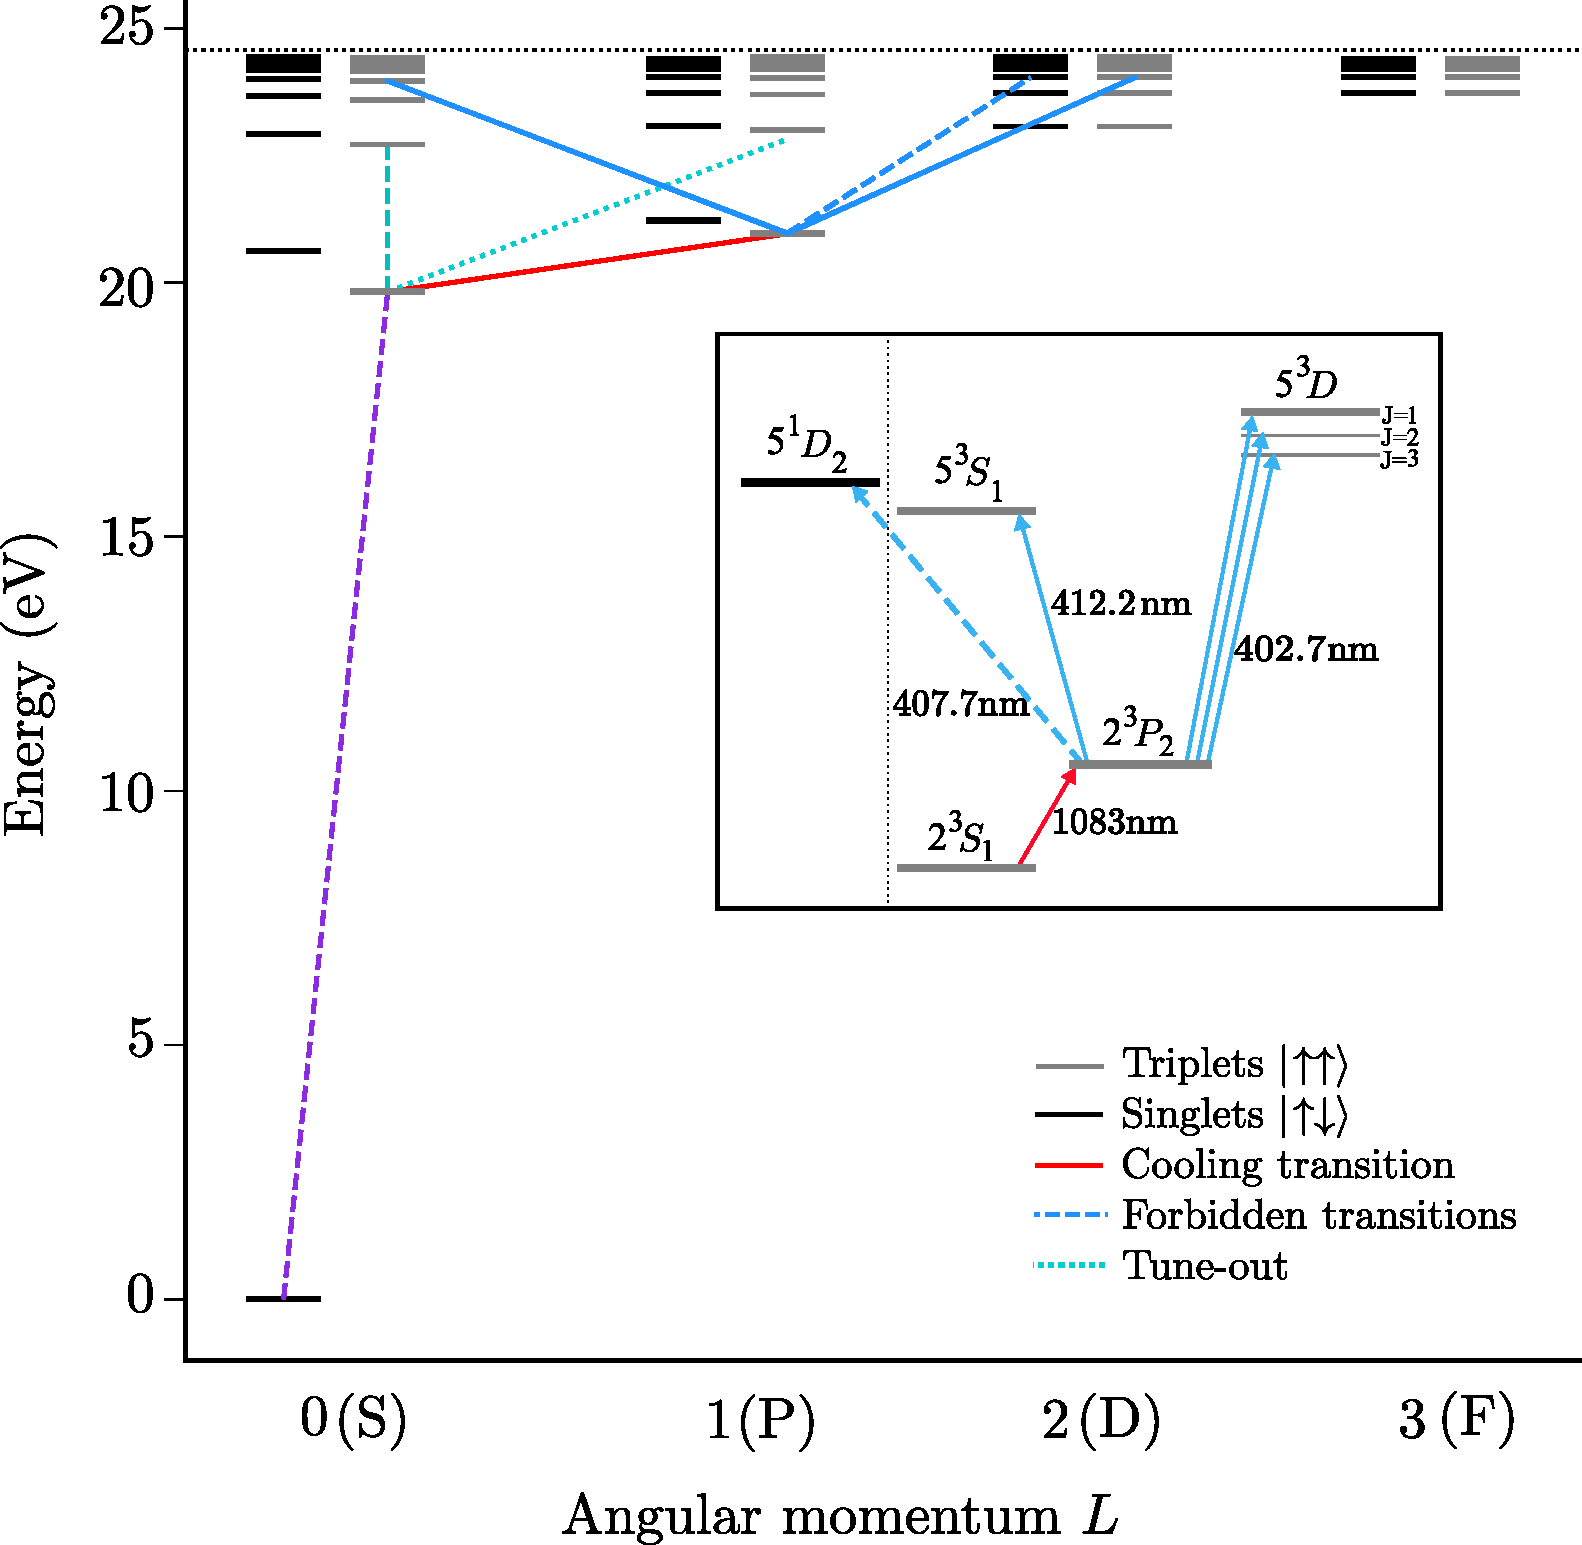
\includegraphics[width=\textwidth]{fig/introduction/full_lvl_diag}
		\caption{A level diagram for $^4$He. Some more words.}
		\label{fig:full_level_diagram}
	\end{figure}

	The astute reader will notice the absence of presentation of an explicit form for the electron wavefunctions in the helium atom.
	Indeed,	helium is not analytically solvable because its eigenfunctions are not separable into a form $\Psi = \psi_1\otimes\psi_2$.
	A variational approach is required for tractable and accurate calculations, which was developed by Hylleraas \cite{Hylleraas1920,Hylleraas1929,Hylleraas1930}.
	In the intervening century, numerical methods for calculating the energy levels and transition rates in the helium atom have kept pace with precision experiments, and have incorporated the effects of relativity, nuclear recoil, and finite optical wavelength. A more detailed survey of recent progress is given in chapter \ref{chap:transitions}.

	

% Fine structure/sublevels; define 'manifold', 'term',' level', 'state' somewhere
	

	\subsection*{Magnetic fields and the Zeeman effect}

	The inclusion of spin introduces another important feature of atomic spectra, the Zeeman effect, whose discovery heralded a `watershed' moment of modern physics.
	The Zeeman effect refers to the phenomenon of spectral line splitting that occurs when an atom is immersed in a DC magnetic field\footnote{Oscillating magnetic fields have other effects on atoms, for example inducing magnetic dipole (or higher order) transitions involving spin-flips.}.
	The interaction energy of an atom in a magnetic field, 
	% \footnote{Along with  the discoveries of X-rays, radioactivity, and the observation that `cathode rays' had a mass-to-charge ratio equal to particles within atoms, now known as \emph{electrons}\cite{FootAtomic}}.
	
	% H spectrum provided observations to challenge class mech, then QM, then RQM, and indeed the current QED
	\begin{equation}
		H = -\text{\boldmath$\mu$}\cdot \textbf{B},
	\end{equation}
	has contributions from both orbital and spin angular momenta ($\textbf{L}$ and $\textbf{S}$, respectively) through the atom's magnetic moment,
	\begin{equation}
		\text{\boldmath$\mu$} = -\mu_B\textbf{L} - g_s\mu_B \textbf{S}.
	\end{equation}
	Working in the $\ket{LSJm_J}$ basis, where $J$ and $m_J$ are the total angular momentum and its z-projection, yields the energies $E_Z = g_J \mu_B B m_J$, where $\mu_B$ is the Bohr magneton..
	The atomic g-factor can be written as
	\begin{equation}
		g_J = \frac{3}{2} + \frac{S(S+1)-L(L+1)}{2J(J+1)},
	\end{equation}
	using the approximate value of the electron g-factor $g_s=2$.
	The eigenstates of the field-free atomic Hamiltonian will be $(2J+1)$-fold degenerate and specified by the $\ket{Lm_L S m_S}$ quantum numbers.
	Adding the magnetic field interaction breaks this degeneracy by introducing off-diagonal terms to the Hamiltonian when expressed in the $LS$ basis,  leading to the Zeeman splitting.
	The field-free and magnetic-interaction terms can be written in a common basis in terms of the Clebsch-Gordan coefficients and then diagonalized, as described in chapter \ref{chap:transitions}.
	The anomalous Zeeman effect arises in triplet states because the inter-level spacing depends on $m$ and $g_J$, which splits spectral lines as well as levels, whereas singlet states have $g_J=1$ and transitions between them do not fan out in the same fashion.
	
	% This distinction, whose explanation was an early victory for quantum mechanics, is illustrated in Figure \ref{fig:ZeemanLines}.
	

	% More than merely splitting lines, the Zeeman effect also induces a polarization-dependence  relative to the quantization axis.
	% The classical dipole envisions only circular polarization is visible along the quantization axis (z oscillation is not visible), but from transverse directions one can see the z oscillation and also the one-dimensional oscillations (eg along x when viewing the y axis) - so in a spatially varying mag field...
	% And we're nearly at the point of being able to project the Stokes vectors into the local field
	


	% RSP [10] ac stark shift -> dipole interaction, can include more levels for better calc [126] 
	% A Askkin acceleration and trapping of particles by radiation pressure, phys rev lett 24, 1970
	% RSP scattering happens [68] 
	% % Grimm, dipole traps
	
	For all the intricacy of atomic structure, life would be very dull indeed were it not for the interactions between them.
	Indeed, the material reality of the world depends, in a sense, less on the structure of its building blocks and more on how they fit together\footnote{This could be said to underpin the transferability of systems from a natural instantiation to analytic or simulated contexts, because there is truth in the \emph{structure} which is independent of the \emph{substrate} - this theme is elaborated in chapter \ref{chap:lattice}.}.
	The varied and central roles of interactions will be revisited in later chapters, traversing the spectrum from isolated, to weakly-interacting, to distinctly many-body systems.
	

\section{Interacting atoms}

	
	Here we briefly review elastic scattering, and then turn to important inelastic scattering processes present in our experiments.
	A detailed primer in atomic scattering physics can be found in the classic texts \cite{PitaevskiiStringari} and \cite{PethickSmith}, with more detail in the latter.
	An exhaustive review of low-temperature scattering studies up to the turn of the millenium can be found in \cite{Weiner99}.
	I focus here on two-body collisions, which are the dominant interactions in the low-density regime of ultracold helium.
	Low densities, which are necessary conditions to minimize the two-body loss processes characteristic to metastable helium, imply that low temperatures are required to achieve high phase space density and reach the degenerate regime.
	Two-body collisions are the crucial enabler for thermalization during the evaporative cooling employed to reach such low temperatures, so long as the relaxation times are shorter than the sample lifetime.

	Neglecting spin-orbit coupling and relativistic effects the two-body scattering problem reduces to the Schr\"{o}dinger equation in the centre-of-momentum frame,
	\begin{equation}
	\left(\frac{\hbar^2}{2m^*}\Delta + V(r) - E\right)\psi(r) = 0,
	\end{equation}
	where $\psi$ is the wavefunction capturing the relative motion of the two atoms	in terms of the separation $r=|\rvec_1-\rvec_2|$ between the particles and the reduced mass $m^*=m_1m_2/(m_1+m_2)$.
	In the asymptotic regime where $r$ is much larger than the scale of the interaction potential $V(r)$, the solution takes the form of a superposition of the initial plane wave and the scattered solution,
	\begin{equation}
	\psi(r) \propto e^{ikz} + f(\theta)\frac{e^{ikr}}{r},
	\end{equation}

	where $k=\sqrt{2m^*E/\hbar}$ is the plane wave-vector of the initial approach and $\theta$ is the angle of scattering from the direction of incidence.
	A general solution can found by expanding $f(\theta)$ into a convenient basis of \emph{partial waves} (spherical harmonics) which are labeled $s,p,d,f,..$ in order of increasing angular momentum.
	In the low-energy limit, $f(\theta)$ is independent of angle and only the spherically symmetric s-wave term contributes, and the limit $f(\theta)\rightarrow-a$ is accordingly called the s-wave scattering length.
	In the millikelvin regime the scattering physics is determined by just a few partial waves \cite{McNamara07}, and in the ultracold (microkelvin or colder) regime only the s-wave scattering channel is significant.
	The total cross section, which is the total probability that a near collision results in particle scattering, approaches $\sigma=8\pi a^2$ for polarized bosons\footnote{For fermion pairs with odd total spin, the cross section tends to zero because of the Pauli exclusion principle, and thus the s-wave scattering length vanishes.} \cite{PitaevskiiStringari,Przybytek05}.
	

	The s-wave scattering length is also an important determinant of the energetics of degenerate matter such as BEC.
	Because BECs are dominated by long-wavelength behaviour, a theoretical treatment can be considerably simplified by considering only the \emph{effective interactions}.
	By formulating the scattering problem in momentum space, the effective interaction strength for low-energy scattering  $g=4\pi \hbar^2 a/m$, also referred to as the pseudopotential, can be found by integrating out the high-frequency modes (also known as the Born approximation).
	This necessarily washes out extremely short-range correlations but makes fairly accurate calculations much more tractable by reducing the size of the basis set used in a calculation.

	In molecular collisions the scattering process will obviously depend on the relative orientation of the molecules.
	In collisions between single atoms, though, there is a more subtle orientation-dependence which arises from the total spin of the two-particle system.
	The three possible configurations between pairs of \mhe~atoms correspond to the singlet $^1\Sigma_g^+$, triplet $^3\Sigma_u^+$, and quintet $^5\Sigma_g^+$ Born-Oppenheimer molecular potentials\footnote{The subscript \emph{g} and \emph{u} are short for \emph{gerade} and \emph{ungerade} (German for even and odd) label the reflection symmetry of the two-body wavefunction.} with total spin 0, 1, and 2 .
	When the atoms are spin-polarized, as \mhe~atoms are when confined in magnetic traps, then the only scattering that occurs is in the quintet channel.
	In low-energy scattering contexts dominated by s-wave scattering, odd partial waves do not contribute to the interaction potential and hence the triplet $^3\Sigma_u^+$ potential is dominated by the quintet $^5\Sigma_g^+$ term for all interactions with nonzero total spin \cite{Leo01}. 
	As such the inter-species scattering lengths $a_{1,1}$, $a_{-1,-1}$, $a_{0,1}$, and $a_{0,-1}$ are all equal \cite{Leo01,Vassen16}.
	The most accurate determination of the s-wave scattering length in these configurations is 7.512 nm \cite{Moal06}, in agreement with calculations performed the year before the measurements \cite{Przybytek05}.
	When the total spin is zero, the singlet potential contributes and so $a_{1,-1}\approx8.8$ nm and $a_{0,0}\approx3.8$ nm \cite{Leo01,Vassen16}.
	In general this thesis will be concerned with interactions between spin-polarized helium atoms and hence will use the abbreviation $a\equiv a_{1,1}$ unless specified otherwise.
	

	A powerful tool available in some cold atom experiments are Feshbach resonances.
	A detailed description is found in \cite{Chin10}, but from an operational standpoint they allow control of the scattering length as $a = \tilde{a}(1-\Delta/(B-B_0))$, where B is the strength of an ambient magnetic field, $B_0$ is the resonance value of the field, $\tilde{a}$ is the value when the field is far from a resonance and $\Delta$ sets the resonance width.
	The scattering length can thus be tuned in size and even in sign.
	However, the stability of a BEC with arbitrary population requires a positive s-wave scattering length.
	Attractive interactions leading to instability and collapse of a condensate with number above a critical value $N_\textrm{cr}\sim\mathcal{O}(a_{ho}/|a|)$, where $a_{ho} = \sqrt{\hbar/m\omega}$ is the length scale of the ground state of the harmonic trap housing the atoms \footnote{In some negative-temperature states created in an optical lattice, a BEC can be stable with attractive interactions \cite{Braun13}.} \cite{PitaevskiiStringari}.
	Switching from stable to unstable configurations permits one to examine condensate collapse (as in the spectacular Bosenova experiments \cite{Cornish00}) and also to explore the BEC-BCS crossover \cite{Bourdel04}.
	The spinless nucleus of $^4$He prohibits coupling of bound states within an $m_J$ manifold from crossing an open-channel threshold, precluding this pathway to a Feshbach resonance \cite{Goosen10}.
	Nonetheless, Feshbach resonances induced by spin-spin interactions between helium atoms have been predicted \cite{Venturi99, Goosen10}, but have not observed to date \cite{Borbely12}.
	In a recent work \cite{Hirsch21}, the authors (including members of the ANU He* lab) describe calculations with a newer method predicting, unfortunately, the absence of Feshbach resonances between $^4$He-$^4$He collisions.
	
	Inelastic scattering processes are those which exchange energy between the internal and motional states of either atom.
	They can be represented as a complex scattering potential \cite{Leo01} which permits losses from on-shell scattering channels.
	An important inelastic process characteristic of metastable noble gases is \emph{Penning ionization} \cite{VassenReview}.
	 This can occur through the decay channels
	\begin{equation}
		\textrm{He}^*+\textrm{He}^*\rightarrow 
		\begin{cases}
			\textrm{He}+ \textrm{He}^+ + e^-&\textrm{(PI)}\\
			\textrm{He}_{2}^{+} + e^-&\textrm{(AI)}
		\end{cases}
	\end{equation}
	wherein the first channel is formally called Penning ionization and the second is  Auto-ionization and the rate of the latter is generally very small in comparison to the former \cite{Muller91}.
	Indeed, the energy of the metastable state is sufficient to ionize any neutral atom (except helium or neon) from its ground state, and underpins the single-atom sensitivity of our solid state detector (described in section \ref{sec:DLD}).
	Aside from attracting intensive study in its own right \cite{Partridge10,Stas06,McNamara07}, this explosive potential was a significant hurdle for researchers attempting to achive Bose-Einstein condensation with helium.
	The density achieved in early magneto-optical traps (MOTs) was limited to some hundredfold less than the alkali-metal MOTs of the day \cite{Bardou92,Kumukura92,Mastwijk98}.
	Helium MOT densities were limited by losses through two-body collisions involving atoms in the $\metastable$ and those excited to the $2\triplet P_2$ state by the trapping beams, as opposed to rescattering pressure as in the case of alkali metals.
	Indeed, while the Penning loss rate constant\footnote{The rate constant $\beta_{i,j}$ for losses via collisions between atoms in states $i$ and $j$ yields an absolute loss rate per volume per time through the product with the respective densities, $\Gamma_{i,j} = \beta_{i,j}n_i n_j$ cm$^{-3}$s$^{-1}$.} between pairs of $\metastable$ atoms is of order $2\times10^{-9}$ cm$^3$/s, the loss rate for $\metastable-2\triplet P_2$  collisions is around $10^{-7}$ cm$^3$/s.
	Thus early MOTs had loss rates which were a population-weighted average of these rates, around $7\times10^{-8}$ cm$^3$/s \cite{Weiner99}.
	Such light-assisted losses  limited the population achievable in MOTs until larger beams and detunings were used \cite{Tol99}.
	The Penning ionization rate is some 20-fold lower at large detunings compared to near-resonant light \cite{Mastwijk98}, reducing this loss rate to the order of $5\times10^{-9}$ cm$^3$/s at large detunings.
	Fortunately, the inelastic scattering cross-sections depend on the molecular potentials in such a way that condensation becomes attainable: When all the atoms are polarized in the either of the $m_J=\pm1$ states, the incoming state has a total spin of 2, whereas the reaction products have a total spin of 1, and so this process is forbidden.
	In reality, it does occur through a weak virtual spin-dipole transition \cite{Shlyapnikov94}, but slowly enough that spin-polarized \mhe~exhibits a $10^4$-fold reduction in the Penning ionization rate.
	At field strengths above 50G, however, the suppression weakens \cite{Shlyapnikov94,Borbely12}.
	Other noble gases also exhibit highly energetic metastable states, but the lifetime and suppression of Penning ionization decreases with increasing mass \cite{Orzel99, Spoden05}.
	Thus helium may be the only noble gas ever to cooled to degeneracy.
	
	% F bardou, O emile, J M courty, C I Westbrook, A Aspect, magneto-optical trapping of metastable ehlium: Collisions in the presence of resonant light, Europhysics letters 20, Dec 1992
	% M Kumakura N Morita, visible observation of metastable helium atoms confined in an invisible/visible resonance trap, japanese journal of applied physics 31, march 1992
	% H C Mastwijk, J W thomsen, P van der straten, A niehaus, optical collisions of cold, metastable helium atoms, physical review letters 80, june 1998

	% \cite{Shlyapnikov94} predicts 1e5x reduction in PI in spin-pol samples; relaxation-induced penning; virtual spin-dipole transitions (induced by spin-dipole interaction) to the zero spin state of the quasimolecule can lift the spin-conservation rule and lead to regular penning ionization	Direc dipole-exchange ionization is also a possibility but dominated by spin-relazation (relaxation-induced penning; virtual spin-dipole transitions to the zero spin state of the quasimolecule can life the spin-conservation rule and lead to regular penning ionization)
	
	
\section{Bose-Einstein condensation}
\label{sec:BEC_theory}

		% M H ANderson, J R Ensher, M R Mathews, C E Wieman, and E A cornell, observation of bose-einstein condensation in a dilute atomic vapor, Science 269, 198-201, July 1995
		% K B Davis, M O Mewes, M R Andrews, N J van Druten, D S Durfee, D M Kurn, W Ketterle, Bose-Einstein condensation in a gas of sodium atoms - Physical Review Letters 75, 3969-3973, Nov 1995
		% C C Bradley, C A Sackett, J J Tollett,  G Hulet, evidence of Bose-Einstein condesnation in an atomic gas with attractive interactions, phyiscal review letters 75, 1687-1690, aug 1995
		% W D Phillips, H Metcalf, Laser deceleration of an atomic beam, Phys Rev Lett 48, 1982
		% Chu et al, three-dimensional viscous confinement and cooling of atoms by resonance radiation pressure, phys rev lett 55, 1985
		% Ch et al, experimental observation of optically trapped atoms, phys rev lett 57, 1986
		% Raab et al, trapping of neutral sodium atoms with radiation pressure, phys rev lett 59, 1987
		% P D Lett et al, observation of atoms laser cooled below the Doppler limit, phys rev lett 61, 1988

	% \subsection{What is a BEC?}
	% Things I might like to put in later: Partition function Z = Tr(\exp(\beta H)), expectation values Tr(O rho)/Z, 

	The fifth state of matter\footnote{The familiar first phases, solid, liquid, and gas, are vanishingly rare in cosmological terms.
	The fourth, plasma, is the state of at leats 99\% of the ordinary matter in the universe \cite{Plasmastuff}.
	Helium comprises about 23\%, most of which being primordial baryons formed during the recombination epoch.}  has a long and storied history\cite{Mukundanote}.
	Interest in BEC was amplified back in the middle of the 20th century when Fritz London proposed that Bose-Einstein condensation was connected to the superfluid phenomenon in liquid helium.
	Nikolay Nikolayevich Bogolyubov formalized this connection and so, historically speaking, helium was the element which hosted the earliest experimental realization of Bose-Einstein condensation, albeit with a very small condensed fraction\footnote{Nikolay was a darling of Russian theoretical physics, receiving his PhD-equivalent qualification at 19 and made important contributions to quantum field theory. In his famous paper on the problem of interacting bosons, his name is transliterated as \emph{Bogolubov}. Bogolyubov and \emph{Bogoliubov} are also common transliterations.}.
	While liquid helium is a rare thing in cosmological terms, BEC may have existed already for millions of years in the superdense quark matter of neutron stars \cite{Haskell18, Martin16,Baym69,Page11}, wresting the claim of cosmic novelty from human hands. 
	Nonetheless, the essentially pure atomic condensates and the emerging study of molecular condensates in laboratory settings are among the most extreme conditions in the universe, and are not believed to occur naturally elsewhere.
	Following the oft-cited seven decades between the initial theoretical descriptions and the experimental realization of atomic Bose-Einstein condensates (BEC) \cite{Davis95,Bradley95,Anderson95}, the field has become quite industrious at the eve of its centenary.
	As pithily put by a review only five years after the Nobel-winning experiments, `Any attempt to review recent progress is out of date as soon as it is published' \cite{Courteille01}.
	This is no less true today, as the number of ultracold quantum gas experiments worldwide\footnote{See \url{everycoldatom.com}} now number nearly 200 and numerous companies have been founded on the promise of selling better sensors and computers using technologies based on BEC physics.
	There are numerous treatments of the theory of Bose-Einstein condensation, for example the classic textbooks \cite{PitaevskiiStringari,PethickSmith} and review articles \cite{Dalfovo99, Yukalov11_basics,Courteille01}.
	The essential background for discussion here draws on these standard sources unless otherwise cited.
	% anquez16 also cites Bogoliubov theory as being used in analysis of quantum phase transitions in spinor condensates


	% There's something to be said here; there is a distinction between the ground state, which is global, and the single-particle states...
	As for what a BEC \emph{is}, there are several workable operational definitions, but a precise and lab-relevant definition is surprisingly elusive.
	The canonical description of Bose-Einstein condensation is the condition where the de Broglie wavelength associated with thermal kinetic energy
	\begin{equation}
		\lambda_T = \frac{h}{\sqrt{2\pi m k_B T}}
	\end{equation}
	is comparable to the interparticle spacing, coinciding with a macroscopic occupation of the single-particle ground state as the de Broglie waves of many bosons constructively interfere.
	This condition can also be restated as the point when the phase space density
	\begin{equation}
		\aleph = n \lambda_T^3
	\end{equation}
	exceeds the critical value of $\zeta(3)\approx2.612$. 
	This is generally introduced of as the point where the volume over which the atoms are `delocalized'  exceeds the average volume per particle, and so the spin-statistics of the particles dictate the deviation from the statistics of an ideal gas.
	Although it is commonly said that at this point the `wavefunctions overlap', the wavefunctions of the individual particles in a trapped gas overlap wherever the wavefunction is supported - that is, throughout the trap.
	Furthermore, the de Broglie wavelength pertains to the wavelength associated with the plane-wave motion of a free particle rather than the spatial scale of the `wavepacket' of a particle, and as given above is defined as the wavelength corresponding to the \emph{average} particle velocity, rather than fully characterizing the ensemble. 
	Thus even above the critical temperature there are many states with long wavelengths who will be populated, and so the `delocalization' picture is not so sharp.
	A more precise criterion is to compute, in the framework of the grand canonical ensemble, the number of particles in the ground state. For a Bose gas this yields
	\begin{equation}
		N_0 = \frac{1}{\exp((E_0-\mu)/k_B T)-1},
	\end{equation}
	where $E_0$ is the ground state energy of the single-particle Hamiltonian and $\mu$ is the chemical potential of an adjoining reservoir. 
	One can then show that, below the critical temperature $T_c$, the ground-state population diverges, corresponding to Bose-Einstein condensation.
	However, in laboratory realizations of BEC, there is no reservoir attached to the system under study, but rather an isolated gas at some finite entropy which contains both the thermal and condensed fractions (if the latter is present). 
	
	Moreover, in the presence of interactions, this criterion faces another issue: the stationary states of an interacting gas of $N$ atoms cannot be written as a product $\ket{\Psi} = \ket{\psi_i}^{\otimes N}$ of single-particle eigenstates $\ket{\psi_i}$.
	That is, while measurements are confined to observables of single particles, the single-particle states are not eigenstates and so it is not sensible to talk of their `macroscopic occupation'.
	The Penrose-Onsager criterion \cite{Penrose56} provides an alternative in terms of the density matrix $\rho$ for the isolated composite system comprised of all the gas particles.
	The single-particle density matrix is then the expected value of the one-body field operator
	\begin{equation}
		\rho^{(1)} = \Tr\left(\rho\hat{\Psi}^\dagger\hat{\Psi}\right),
	\end{equation}
	whose eigenvalues $p_{l}^{1}$ give the occupation probability of the $l^{\rm th}$ eigenvector of $\rho^{(1)}$.
	The eigenvectors themselves are the single-particle modes (which may be, in general, some superposition of the non-interacting eigenstates).
	If any eigenvalue $p_{l}^{i}$ is proportional to $N$ in the limit $N\rightarrow\infty$, then the system is said to have undergone Bose-Einstein condensation (or, simply, \emph{condensed}) into the $l^\textrm{th}$ mode.
	Of course, real systems are subject to atom losses and heating, violating the assumptions of equilibrium underpinning both the approaches above.
	
	This is all to illustrate the point that the real world is full of intricacies and the `intuitive' pictures of BEC, despite being useful pedagogical tools, can skirt around some important physical features.
	Ultimately though, this is a thesis concerned with experiments, and we shall say little more than remarking on the compelling agreement between abstract and actual condensates irrespective of the preceding issues.
	Indeed, the Penrose-Onsager criterion has been shown to be a good characterization of a non-Hermitian polariton condensate \cite{Manni12} in that off-diagonal long range order (i.e. phase coherence) emerges along with the growh of a single eigenvalue of the one-body density matrix.
	As the saying goes, if it interferes like a condensate \cite{Andrews97} , undergoes number fluctuations like a condensate \cite{Kristensen19},  has HBT correlations like a condensate \cite{Schellekens05,Jeltes07}, Kibble-Zureks like a condensate \cite{Anquez16}, and quacks like a condensate \cite{Duck01}, then it probably \emph{is} a condensate.

	While most atomic condensates, and all of those in this thesis, are trapped in non-uniform potentials, many important features of condensates are easier to state for homogeneous systems.
	One can usually extend calculations to harmonically trapped systems by a local density approximation, wherein one performs a density-weighted average across a condensate, considering each volume element as a homogenous condensate in its own right.
	Thus, for the most part the following discussion will focus on homogeneous systems for simplicity's sake.
	I present some particular results in the case of a harmonically trapped gas at the end of this section.

	% \todo{ODLRO links}
		% https://physics.stackexchange.com/questions/79846/what-is-off-diagonal-long-range-order-in-superfluid
		% https://arxiv.org/abs/1804.04084

	% distinction worth making; the ground state is a global property of the configuration.
	% Interactions mean it is not the same as the product of single-particle ground states: I mean, it *is* actually in this case, I think, but the ground states are not solutions of a free hamiltonian (I guess they are in the bogo pictures though??)


	% Potential for historical note about liquid helium
	
	%  Potential resolution; Mastsubara (1955) A new approach to quantum-statistical mechanics, Progress of Theoretical Physics vol 14, no 4
	% Many characteristic features predicted for Bose-Einstein condensates have been observed in ultracold trapped gases.
	
	% Something something grand-canonical ensemble; role of chemical potential; tracing out reservoir
	% We have the other formlation, \rho = \exp(\beta \hat{H});
	\subsection*{Bogoliubov theory}
	The fundamental theoretical object of interest is the Hamiltonian of a bosonic quantum field with two-body interactions $\hat{H} = \hat{K} + \hat{I}$, with kinetic part
	%mark
	\begin{equation}
		\hat{K} = \int\left(\frac{\hbar^2}{2m}\nabla\hat{\Psi}^\dagger(\textbf{r})\nabla\hat{\Psi}(\textbf{r})\right)d\textbf{r}
		\label{eqn:ham1}
	\end{equation}
	and the interaction term
	\begin{equation}
		\hat{I} = \frac{1}{2}\int\left(\hat{\Psi}^\dagger(\textbf{r}')\hat{\Psi}^\dagger(\textbf{r})V(\textbf{r}'-\textbf{r}) \hat{\Psi}(\textbf{r}')\hat{\Psi}(\textbf{r})\right)d\textbf{r}'d\textbf{r}
		\label{eqn:ham2}
	\end{equation}
	where $\Psi(r)$ are the field operators subject to the bosonic commutation relations
	\begin{align}
		[\Psi(r),\Psi^\dagger(r')] &= \delta(r-r')\\
		 [\Psi^\dagger(r),\Psi^\dagger(r')]&=[\Psi(r),\Psi(r)]=0.
	\end{align}	
	We can then write the field operator in the suggestive form	
	\begin{align}
		\hat{\Psi} &= \psi_0 \hat{a}_0 + \sum_{i\neq0}\psi_i \hat{a}_i
	\end{align}
	in terms of an orthonormal basis of single-particle modes $\psi_i$ and corresponding field operators $\hat{a}_i$.
	In doing so we distinguish $\pvec=0$ as the condensed mode, and say that condensation occurs when $N_0=\langle\hat{a}^\dagger_0\hat{a}_0\rangle =\mathcal{O}(N)$.
	The observation that the condensed mode has a population of order $N$ means that in the thermodynamic limit ($N\rightarrow\infty,~V\rightarrow\infty$), one particle here or there will not really make a measurable difference.
	% More quantitatively, one could say $\hat{a}_0\psi_0 = 
	This argument can be expressed quantitatively as the Bogoliubov approximation wherein the annihilation and creation operators for the condensed mode are replaced with complex numbers as per
	\begin{equation}
		\hat{a}_0 = \sqrt{N_0}e^{i\alpha}, \hat{a}_0^\dagger= \sqrt{N_0}e^{-i\alpha}, 
	\end{equation}
	which permits the condensate wavefunction to take the form
	\begin{align}
		\hat{\Psi} &= \sqrt{N_0}e^{i\alpha} \psi_0 + \delta\hat{\Psi}\\
					&= \Psi_0 + \delta\hat{\Psi}
	\end{align}


	% Where  $\sqrt{N_0}e^{i\alpha}$ is the \emph{order parameter} which gives the amplitude of the condensate wavefunction and $\psi_0$ is some self-consitent defn of the condensed mode, however one gels the atom-density-matrix defn with the bosonic field...
	

	% usuall The eigenfunctions of the non-interacting(?) case can be used to express the field operator $\Psi(r) = \sum_i \phi(i) \hat{a}_i$ in terms of the creation operator, which obeys similar commutation relations.
	% This then leads to a similar separation of the field operator into the condensed and noncondensed part,
	% % $$
	% % \Psi(r) = \phi_0\hat{a}_0 + \sum_{i\neq0}\phi_r(r)\hat{a}_i,
	% % $$
	% % Does bogo assume $[\hat{a}_o,\hat{a}^{\dagger}_0] = 0$? 
	% % form is then $\Psi(r) = \Psi_0(r) + \delta\Psi(r)$ where the first term on RHS is the complex fn $\sqrt{N_0}\phi_0$ and the last term is a sum over other modes.
	
	% %%See also; assuming \Psi = \phi + \hat{\psi} with \int|phi|^2 >> \langle\psi^\dagger\psi\rangle permits discarding third-and-higher order terms in the full bosonic field hamiltonian, leading to GPE...
	% how relates to Born approx?
	The first term is the condensate wavefunction (the \emph{mean-field} term), and the second corresponds to the population of non-condensed modes thanks to the effect of interactions, which are captured by the quasiparticle picture sketched in the next section.	The emergence of a condensate has many of the hallmarks of a classical phase transition: kinetic effects are necessary to redistribute energy and reach steady-state; a unique critical temperature $T_c$ exists; below $T_c$ an \emph{order parameter} takes on a nonzero value; and condensation is equivalent to the spontaneous breaking of a U(1) gauge symmetry \cite{Yukalov11_symmetry}.
	Above the critical temperature, $|\Psi_0|=0$, and in general it exhibits a discontinuous derivative at the critical temperature.
	Hence, in the Landau-Ginzburg framework, condensation is a second-order phase transition\footnote{In the Ehrenfest picture one is instead concerned with the number of times one must differentiate some state function (e.g.
	specific heat, compressibility, pressure, free energy) before finding a discontinuity at the critical point.
	In this picture, the transition is first-order as one has continuous state functions with discontinuous derivatives.}.
	The other hallmark of Landau-Ginzburg phase transitions is the spontaneous breaking of symmetry as one crosses from the disordered to the ordered phase (as when a solid breaks the translational symmetry of the fluid phase).
	Condensates do exhibit such symmetry breaking: The Hamiltonian has a $U(1)$ gauge symmetry, but the ground state of a condensate spontaneously chooses a fixed but unpredictable phase $\alpha$.
	By interfering two independently prepared condensates, one observes interference fringes \cite{Andrews97}, and indeed, the fringe locations will change with each realization and measurement.
	More directly, one can interfere light leakage from a reservoir-coupled photon condensate against a reference beam, and observe that phase jumps occur in the output when the condensate field drops to zero.
	That is, the re-emergence of the condensate is heralded by the selection of a new, specific, phase, apparently uncorrelated with the phase that existed before it \cite{Schmitt16}.
	
	
	Symmetry breaking is a subtle point discussed infrequently in standard textbooks.
	It happens that one can substitute complex numbers for the field operators,  even when $\langle N_0\rangle \rightarrow 0$ and still obtain correct results \cite{Ginibre67}.
	That is, condensation is not necessary for the Bogoliubov approximation to be valid.
	However, it \emph{is} the case that the onset of condensation coincides with the ground state breaking\footnote{This is sometimes called `breaking the gauge symmetry'.
	This is a misnomer, as a gauge symmetry is a property of the theory, not a state, and all consistent theories must be gauge symmetric throughout.
	These subtleties are discussed at length in lucid terms in \cite{Poniatowski19}.} the $U(1)$ symmetry \cite{Suto05}.
	
	% That this coincides with the validity of the `coherent state' approximation is quite profound: Like the transition from the quantized electromagnetic field to the Maxwell equations, BEC has the flavour of a classical field but one which is consitued by matter which has dispersed in some delocalized state.
	% The interactions between atoms present a marked departure from the physics of the electric field, however, and yet the system remains in the grasp of human theorists thanks to the Bogoliubov approximation, which I introduce here and examine experimentally in chapter \ref{chap:QD}.
	% %  First-order phase transition as the chemical potential has a discontinuous derivative \cite{Ykalovreview}, cf ehrenfest critioerion of discontinuous derivative of a state function; the ginzburg-landau classification is in terms of the order parameters; BEC is a second-order transition as the order parameter is continuous with a discontinuous derivative.
	% % Penrose and Onsager generalized the definition of condensation to include interacting particles and non-uniform systems.
	%  In fact, the Bogoliubov picture of superfluidity actually refers to a condensation of non-interacting collective bosonic modes, rather than the condensation of the constituent atoms.
	% The definitions coincide fairly well.../
	% % NB most BEC theory most simply stated for homogeneous systems, so will consider these initially, and return to a few remarks about harmonically trapped gases at the end of the section.


	% Actually in the following, one starts from the full second quantized hamiltonian and assumes smooth density in the born approx to get to the  GPE.
	% The variational approach is just an alternative and need not be included.
	
	
	
	\subsection*{Harmonically trapped condensates}

	Turning back toward harmonic gases, we can begin from the full Hamiltonian (Eqns.
	(\ref{eqn:ham1},\ref{eqn:ham2}) and produce an effective Schr\"{o}dinger equation.
	By assuming slow variations in the density, integrating out short-wavelength modes as in the Born approximation, one can derive the Gross-Pitaevskii equation (GPE),
	\begin{equation}
		i\hbar\frac{\partial \Psi_0(r,t)}{\partial t} = \left(-\frac{\hbar^2\nabla^2}{2m} + V(r,t) + g|\Psi_0(r,t)|^2\right)\Psi_0(r,t).
		\label{eqn:GPE}
	\end{equation}
	which is valid for arbitary interactions dominated by the s-wave scattering length.
	 If one further assumes that the condensate density varies on scales larger than the healing length $\xi = \hbar/\sqrt{2mgn}$, one can make the Thomas-Fermi approximation and ignore the kinetic term in the GPE, whereby the condensate density profile can be written as

	
	\begin{equation}
		n(\textbf{r}) = \frac{\mu-V(\textbf{r})}{g},
	\end{equation}
	where $\mu$ is the chemical potential.
	The chemical potential for the harmonically trapped condensate also fixes the average energy per particle as
	\begin{equation}
		\mu = \frac{7}{5}\frac{E}{N} = \frac{\hbar\bar{\omega}}{2}\left(\frac{15 N a}{a_{ho}}\right)^{2/5} ,
	\end{equation}
	recalling $a_{ho} = \sqrt{\hbar/m\omega}$ is the length scale of the ground state of the harmonic oscillator.
	For a Bose gas confined in a harmonic potential of the form
	\begin{equation}
		V = \frac{1}{2} m \omega_x^2 x^2 + \frac{1}{2} m \omega_y^2 y^2 + \frac{1}{2} m \omega_z^2 z^2,
	\end{equation}
	the condition $\mu-V(\textbf{r})=0$ determines the boundary of the condensate, giving the Thomas-Fermi radii $R_i = \sqrt{2\mu/m \omega_i^2}$, where $i\in\{x,y,z\}$.
	This produces the famous inverted-parabola density profile with a peak density of
	\begin{equation}
		n_0 = \frac{1}{8 \pi}\left( (15N_0)^2 \left(\frac{m \bar{\omega}}{\sqrt{a \hbar}}\right)^{6}\right)^{1/5}.
		\label{eqn:n0}
	\end{equation}
	The Thomas-Fermi approximation is valid when $N a/a_{ho}\gg1$. 
	This is when the mean-field energy significantly outweighs the kinetic term.
	The phase space density for condensation is achieved at the (ideal) critical temperature 
	\begin{align}
		T_c^{0} &= \frac{\hbar \bar{\omega}}{k_B}\left(\frac{N}{\zeta(3)}\right)^{1/3}\\
				&\approx0.94\frac{\hbar \bar{\omega} N^{1/3}}{k_B}.
	\end{align}
	where $\bar{\omega}=(\omega_x\omega_y\omega_z)^{1/3}$ is the geometric mean of the trapping frequencies, and the condensed fraction below the critical temperature is 
	\begin{equation}
		\frac{N_0}{N} = 1 - \left(\frac{T}{T_c^{0}}\right)^3.
	\end{equation}
	The rest of the population, occupying excited single-particle states, is called the thermal fraction.
	The population $N_T$ of the thermal fraction saturates as $\frac{N_T}{N} = \left(\frac{k_B T}{\hbar \bar{\omega}}\right)^3$ in a non-interacting Bose gas, wherein any atoms added to the gas fall into the condensate mode, regardless of the density of the gas.
	Real gases generally don't show such a feature, and this bifurcation is corrected by including the effect of interactions on the thermodynamics of the Bose gas.	 
	Interactions between particles reduce the critical temperature in a harmonic trap, which can be understood in terms of repulsive interactions reducing the density at a given temperature and thus requiring a lower temperature to achieve a give $\aleph$.
	The resulting shift in the critical temperature can be supplemented with a correction for the finite population of the condensate and written as
	\begin{equation}
		\frac{\delta T_c}{T_c^{0}} = -1.3 \frac{a}{a_{ho}} N^{1/6} -0.73\frac{ \langle\omega\rangle}{\omega_{ho} N^{1/3}}
	\end{equation}
	where the latter term, the correction for finite atom number, includes the arithmetic mean trapping frequency $\langle\omega\rangle$ and vanishes in the thermodynamic limit $(N\rightarrow\infty,~V\rightarrow\infty,~N/V$ finite).
	These deviations from ideal behaviour have been observed in experiments \cite{Tammuz11,Smith11}.

	% For an ideal gas, this is the expected fraction of the population in the ground state of the trap.
	As for the practical production of condensates, much quality literature has been written on the theory and techniques of atomic cooling employed to reach degeneracy.
	These days, such techniques are standard across hundreds of laboratories and so space will not be spared for their general consideration here.
	The curious reader is directed to \cite{MakingProbingUnderstanding,Courteille01,MetVdS, TychkovThesis} for detailed discussions.
	Rather, in the next chapter I discuss the specifications of the apparatus I used in the course of this research. 
	
\subsection{Cooling techniques}
	\label{sec:doppler_basics}
	In brief, both BEC machines discussed in this thesis exist to achieve magnetic trapping of metastable helium in ultra-high vacuum (UHV) conditions, and from there apply further operations as required by the science at hand.
	Magnetic trapping is required because the limits of optical cooling are too hot to achieve degeneracy with the densities realizable with optically trapped helium.
	However, optical cooling is a necessary first stage of cooling to reach the cold (millikelvin) regime before evaporatively cooling to the ultracold (microkelvin) regime en route to degeneracy in the nanokelvin regime.
	Doppler cooling is the most-used optical cooling technique in this thesis for two main reasons.
	First, helium's spinless nucleus means it has no hyperfine structure and precludes some other forms of sub-Doppler cooling.
	Second, Doppler cooling is sufficient to reach phase space densities high enough to seed evaporative cooling sequences which achieve condensation. 
	
	% H F Hess, Evaporative cooling of magnetically trapped and compressed spin-oolarized hydrogen, Physical Review B 34, 3476-3479, Sept 1986
	% W Ketterle and N J van Druten, Evaporative cooling of traped atoms, advanes in atomic molecular and optical physics 37, 181-236, 1996
	% O J Luiten, M W reynolds, J T M Walraven, Kinetic theory of the evaporative cooling of a trappe dgas, Physical Reveiw A 53, 381-389 Jan 1996
	Doppler cooling effectively produces a velocity-dependent force by exploiting both radiative pressure and the Doppler effect, which I illustrate here with reference to a two-level atom with resonant frequency $\omega_0$.
	An atom moving with velocity $\vec{v}$ with respect to the source of a laser (approximated as a plane wave with wavevector $\vec{k} = \omega/c$ in the reference frame of the laser emitter) will see a radiation field with a Doppler-shifted frequency $\omega' = (1 - \vec{k}\cdot \vec{v}/c)\omega$.
	If the laser is detuned from the transition one has the resonance condition $\vec{k} \cdot \vec{v}/c = (1 - \omega_0/\omega)$, hence if the detuning $\Delta = \omega-\omega_0$ is negative (i.e. the laser is \emph{red} of the resonance) then the light is Doppler-shifted into resonance in the atomic frame for some $\vec{k} \cdot \vec{v}<0$, i.e. when the atom is moving toward the source of the laser. 
	When the atom absorbs a photon and is excited to the upper state of the transition it acquires the photon recoil momentum $\vec{p} = \hbar \vec{k}$.
	If the laser is red-detuned then this impulse opposes the atomic motion along the $\vec{k}$ direction and slows the atom down.
	The atom eventually decays to the ground state on a timescale $\tau = 1/\Gamma$ where $\Gamma$ is the excited-state linewidth.
	The emission events (at a rate $\Gamma$) are isotropic and so the integrated momentum imparted from the many emission recoils is zero.
	The atom is then excited again at a rate $\Gamma_{sc}$ (the real part of Eqn. \ref{eqn:lorentzian}), which can be written 
	\begin{equation}
		\Gamma_{sc} = \frac{s}{2 }\frac{\Gamma}{1 + s + (2\delta/\Gamma)^2}
	\end{equation}	
	in terms of the (atom-frame) detuning $\delta$ and $s=I/I_\textrm{sat}$, where the saturation intensity $I_\textrm{sat} = \pi h c \Gamma/(3\lambda^3)$ is $0.167$ mW/mm$^2$ for the cooling transition in \mhe~\cite{BaldwinReview}.
	The cycling absorption-emission events culminate in an effective force $\vec{F} \approx \Gamma_\textrm{sc}\hbar\vec{k}$ (when $\Gamma_\textrm{sc}>\Gamma$) called the \emph{radiative force}. 
	The scattering rate $\Gamma_\textrm{sc}$ depends on the detuning, hence the radiative force inherits a velocity-dependence via the Doppler effects and so is occasionally called \emph{optical molasses} because it is a friction-like force that reduces the atomic kinetic energy.

	% bergeman93 quantum calculations for one-dimensional laser cooling
	% castin89 limits of laser cooling in 1D
	% castin91 theory of sisyphus cooling(polz gradient?)
	% doery94 using 1083nm transition to look at lattice effects in optical molasses

	The fundamental temperature limit for laser cooling is the \emph{recoil limit} set by the relation $k_B T = \hbar^2k^2/2m$, where $k$ is the wavevector of the cooling light.
	This is the energy scale fixed by a single-photon emission, and is about 2 $\mu$K for Helium.
	While this is too hot to achieve condensation in the traps considered in this thesis (whose critical temperature is about 1 $\mu$K), we generally only use laser cooling down to the \emph{Doppler limit}.
	The latter is given by $T = \hbar\Gamma/2 k_B\approx 38~\mu$K and corresponds to the minimum velocity difference which can be distinguished by the cooling laser.
	In practise this is set by the linewidth $\Gamma$ of the cooling transition (1.6MHz for the $2\triplet S_1 - 2\triplet P_2$ transition), as the laser linewidth is smaller by about an order of magnitude \cite{Shin16}.
	These limits of optical cooling mean that laser cooling of helium to the ground state of our traps is not possible.
	Furthermore, helium has a spinless nucleus and thus no hyperfine structure, precluding the polarization-gradient cooling employed in alkali atoms.
	Fortunately, condensation is achievable via evaporative cooling in magnetic traps (and in an optical dipole trap, as discussed in chaper \ref{chap:lattice}).

	The machinery used to cut the pathway from room temperature to degeneracy is described in the next chapter. 